
\section{Challenges and Design Rationale}
\label{sec:hublink_design_rationale}

During the development of the HubLink approach, we faced several challenges that influenced key design choices. In this section, we outline the reasoning behind these decisions. We begin by explaining our choice of an embedding-based retrieval approach. Next, we discuss the motivation for decomposing each \texttt{HubPath} into multiple levels. We then describe the benefits of extracting components from the input question as a pre-processing step. Following that, we explain the role of a diversity ranker in enhancing the relevance of retrieved \texttt{HubPaths}. We also justify the use of weighted averaging when calculating the overall score of a hub. Additionally, we provide our rationale for incorporating a linking procedure and present the reasoning behind splitting the HubLink approach into two distinct strategies. Finally, we present the rationale behind the prompts that were engineered to realize the approach.

\subsection{Using Embedding-based Retrieval}

One significant challenge that we had to solve was the efficient retrieval of relevant graph data. One major reason is the exponential growth of candidate subgraphs as the graph size increases. This means that the number of graph elements that need to be considered during retrieval grows exponentially. This presents a substantial challenge because \gls{kgqa} retrieval algorithms must ensure semantic relevance between the query and graph structures. This task is particularly difficult due to the high dimensionality of textual data within the nodes and edges of the graph. Consequently, this requires the development of heuristic search algorithms capable of efficiently exploring and retrieving relevant graph elements. \cite{peng_graph_2024,hu_grag_2024} 

In addition, a suitable user experience is important. This requires balancing both the runtime and the costs of the approach. 

We addressed the size of the graph by transforming the information of the graph into a vector space using a pre-trained embedding model. This enables the quick identification of relevant information through an \gls{ann} search between the stored vectors and the search query vector. By applying this technique, we reduced the complexity of the problem from having to deal with the size of the graph to dealing with how effectively we can query relevant vectors from the vector store.


\subsection{Decomposing HubPaths to Multiple Vector Levels}

It is challenging to consider both textual information and topological graph structures during graph retrieval. This is important because textual data convey information, while structural data describe the relationships between them. This requires the approach to account for both semantic information in the text and structural information in the graph. This challenge is further complicated by the fact that textual graphs often contain vast amounts of information, of which only a small portion is actually relevant to answering the query. Therefore, this problem requires the development of algorithms that can understand both textual and structural information and efficiently filter out irrelevant graph elements without losing critical information. \cite{peng_graph_2024,hu_grag_2024}

We encountered this challenge during the transfer of knowledge from the graph to the vector space as we needed to decide how to best store both textual and structural information. We approached this issue by generating textual path descriptions with an \gls{llm} that captures both the information conveyed in the graph nodes and the relationships between them.

However, just converting the paths to textual descriptions and transforming them into dense vectors did not completely solve this issue. We found it to be important to consider the granularity of the vectors stored in the vector store. This is because irrelevant details can overshadow potentially relevant information. In other words, if too much information is loaded into a single vector at once, the similarity to the search query may decrease due to the presence of irrelevant data, causing relevant information to be missed. Conversely, if too little information is transferred into the vector, important details might be neglected, likewise reducing the similarity to the query. Thus, there exists a trade-off with respect to the amount of information embedded within a vector. Both an excess and a deficiency of information can result in relevant data not being found.

To address this trade-off, we decided on storing each \texttt{HubPath} in four different content levels, as detailed in Section~\ref{sec:hublink_hubvector_definition}. With this design decision, we reduce the risk that irrelevant data overshadows relevant data because there now exist multiple vectors, each representing a different level of content that can potentially match the question or its components. This design decision is closely related to the decision to extract components from the questions asked, which we discuss below. 

Furthermore, we store the textual description and the triples of the path as metadata for each vector. This is important because the embedded text of the vector (other than the path level) loses context. To solve this, vectors are used for similarity matching during retrieval, and the answer is generated using the triples and path description of the associated \texttt{HubPath} to ensure enough context is included. A drawback of this approach is that each \texttt{HubPath} appears multiple times in the index (once for each content level). This can result in the same information being returned multiple times during retrieval without any added value. To prevent this, we apply a \emph{deduplication} process that is realized by storing the unique hash value with each \texttt{HubPath} as additional metadata. During retrieval, we then ensure that for each hash value, only the top-scoring vector is considered.

\subsection{Extracting Components from Questions}

It is challenging to address the varying complexity of questions as they can range from simple to highly complex. Basic examples include: \enquote{Who are the authors of the paper?} while more complex queries might be: \enquote{Which reference architectures for cloud-native applications based on Kubernetes were published in 2020?} Complex questions consist of multiple aspects that need to be considered individually. During the design of HubLink, it became apparent that it is unlikely to find all relevant information for a complex question within a single path. As a result, doing the nearest-neighbor search using only the embedding of the question leads to insufficient results.

Our solution to this problem is to decompose the question into its individual components representing various semantic elements. Referring to the example question above, these components could be \emph{reference architectures}, \emph{cloud-native applications}, \emph{Kubernetes}, and \emph{2020}. Because we store the paths in the index at multiple granular levels, we increase the chances of achieving higher similarity scores using the extracted components. This is feasible because smaller vector units contain less information, enabling more accurate matching of specific content without reliance on the surrounding context.

\subsection{Using Hubs to Semantically Store Information}

\begin{figure}[t]
    \centering
    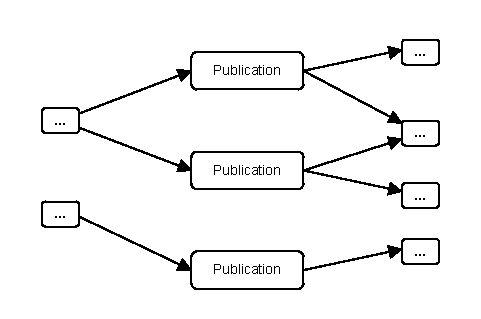
\includegraphics[width=0.75\textwidth]{figures/figures-RKG_structure.drawio.pdf}
    \caption[Example Structure of an RKG]{Example structure of an \gls{rkg}. Here, the information of interest is gathered as a subgraph around nodes of type \emph{Publication}. HubLink uses these subgraphs by encoding them as Hubs to perform targeted inference.}
    \label{fig:rkg_structure}
\end{figure}

When retrieving data from a graph, it is important to ensure that the relationships between information are retained correctly to avoid losing valuable data. This can be challenging, as it is not always clear how much of the surrounding information is actually needed \cite{peng_graph_2024,hu_grag_2024}. Our solution to this challenge is to decompose the graph into distinct \texttt{Hub} structures. This design choice is informed by the way information is organized within an \gls{rkg}. As observed by \textcite{verma_scholarly_2023}, an \gls{rkg} stores scientific data through research entities. Due to the inherent structure of graphs, related data tends to cluster around these entities. In this setup, the research entities act as roots, aggregating scientific information through their neighboring nodes. 

\autoref{fig:rkg_structure} illustrates this concept. It shows entities of the \emph{Publication} type that inherently store scientific information about the publication around them. In this case, each publication entity serves as a root, with its associated data stored in the surrounding nodes. Given that questions in scholarly \gls{kgqa} typically target information related to research entities, this natural clustering is exploited in the retrieval strategy of HubLink. We refer to this cohesive unit of information as a \texttt{Hub}, where each hub is based on a root node and encompasses all semantically related information accessible through paths originating from it.

Encoding these hubs in a vector space requires careful consideration of two key aspects: a) the significance of a node relative to the root node of the hub, and b) the preservation of relationships among the nodes within the hub. To meet both criteria, we consider all directed paths within the hub that start at the root and lead to end nodes. These paths are referred to as \texttt{HubPaths}. At the core, each \texttt{HubPath} represents a directed path within a hub that starts at the root entity of the hub, follows the direction of the graph, and either a) continues to the end of the graph, b) reaches a predetermined maximum length, or c) encounters a new root node of another hub. The idea of a \texttt{HubPath} is that the information on the path shares a common semantic meaning and should be encoded together in the vector space. Therefore, each \texttt{HubPath} is converted to vectors during indexing and stored in a vector database.


\subsection{Applying a Diversity Ranker on the Triple Level}

During development, we encountered an issue caused by retrieving triple-level vectors from the index. Since it is common that multiple triples $(s,p,o)$ share the same subject $s$, this leads to a situation where many irrelevant triples receive a high similarity score simply because they share the same subject. This creates a problem during retrieval in which only a fixed number of \texttt{HubPaths} are selected per candidate hub.
% The retrieved paths often add no value to answering the question because they all have the same subject entity, which by itself has a high relevance to the query, but the remaining information in the triple has not.

To illustrate this, consider the following question: \enquote{Which authors does the paper with the title 'A Complexity Metric for Microservices Architecture Migration' have?}. When this question is processed, it is decomposed into several components, one of which includes the paper title. Then, a similarity search is performed using these components. If the graph contains many triples where the title is the subject, these triples may dominate the top results due to the strong subject match, regardless of whether their predicates and objects are actually useful for answering the question. This effect can crowd out more relevant triples, such as those identifying the authors, from the top-k ranked \texttt{HubPaths} for a hub.

To mitigate this issue, we introduce a \emph{Diversity Ranker}. This component penalizes triples whose subject has already been encountered, thereby encouraging a more diverse set of \texttt{HubPaths} in the results. This increases the chances of retrieving paths that contribute novel and useful information. 

\subsection{Using Weighted Averaging for Scoring of Hubs}

In earlier stages of development, we calculated the score of a hub by taking the average of all associated \texttt{HubPath} objects. However, this approach revealed an issue that led us to adopt a weighted mean instead. Originally, the unweighted hub score was calculated as:

\[
\text{Score}(Hub) = \frac{1}{n} \sum_{i=1}^{n} \text{Score}(h_i), \quad h_i \in \mathcal{H}
\]

Here, \( \mathcal{H} \) denotes the set of all \texttt{HubPath} objects for a given hub, \( h_1, \dots, h_n \) are the individual paths, and \( n \) is the number of these paths. The main drawback of this method is that all paths are treated equally, regardless of their individual relevance. As a result, a hub with many average-quality paths could end up with a higher total score than a hub that has fewer but highly relevant paths. This leads to a situation where important paths with high scores are overshadowed by a large number of less relevant ones, even though they might be critical for the overall quality of the hub. To address this issue, we now use a weighted mean, where paths with higher scores contribute more significantly to the overall score of the hub. Formally, let \( \vec{s} = [s_1, s_2, \dots, s_n] \) be the list of scores of all paths for a given hub. The weights for this new calculation are computed as follows:

\[
w_i = \exp(\alpha \cdot s_i)
\]

The final weighted score of the hub is then given by:

\[
\text{Score}(Hub) = \frac{\sum_{i=1}^{n} w_i \cdot s_i}{\sum_{i=1}^{n} w_i}
\]

The parameter \( \alpha \) controls the extent to which high path scores are emphasized. Furthermore, this parameter can be fine-tuned to adapt to any given context. 


\subsection{Enriching Hubs by Linking to External Data}

Although representing information as a graph introduces structure and emphasizes semantic relationships, it also comes with a trade-off: a loss of textual detail. This occurs because textual content must be adapted to the \gls{rdf} format, which fragments information into triples, each capturing only a small portion of the original narrative. The goal of the linking process in HubLink is to complement the structured graph data with additional, richer context from external sources. This should enhance answer generation by providing more complete and informative responses.


To illustrate, consider a literature search scenario in which individual papers serve as the hub objects. Each hub is associated with a unique identifier, typically the DOI of the paper. This identifier enables the retrieval of additional information beyond what is captured in the graph. For example, we may connect to an external vector store that holds embeddings of the full-text from papers. Once relevant hub candidates are identified, the linking process uses their DOIs to perform targeted nearest-neighbor searches on these text embeddings. The returned text segments are then used to enrich the knowledge of the corresponding hubs. By combining structured graph data with context-rich textual extracts, this process can lead to more comprehensive and nuanced answers. In addition, it supports transparency in the retrieval process, as the enriched responses can be directly traced back to their source documents.



\subsection{Providing Two Different Retrieval Strategies} 

During the development of HubLink, we decided to implement two different retrieval strategies. This decision was driven by a trade-off that emerged during development. By introducing both strategies, we allow users to choose the strategy that best suits their specific use case. In the following, we take a closer look at this trade-off.

The first approach, \emph{direct retrieval}, enables fast retrieval using the vector index to quickly identify semantically similar content. Although this method is efficient and scalable, it becomes less effective in retrieving localized information as the size of the index grows. When multiple contexts from different sources share semantic similarity with the query, they may all be retrieved, regardless of whether they are relevant to the specific intent of the question. This can be problematic for questions that are meant to target particular segments of the knowledge graph.

To mitigate this limitation, traditional search systems often use metadata filters (e.g., research field, publisher, publication year) to narrow the scope of search results. HubLink incorporates a similar principle in its second strategy, \emph{graph traversal retrieval}. In this approach, a specific entry point in the graph, referred to as a topic entity, is used to constrain the search to a relevant subregion of the graph. Without such a focus, the system would need to search the entire graph, increasing the risk of retrieving irrelevant information from unrelated areas. Consequently, the topic entity effectively acts as a filter, making this strategy particularly valuable in large-scale graphs containing millions of nodes.

However, using the \emph{graph traversal retrieval} strategy comes with the drawback that a topic entity must be known or inferred. In some cases, such an entity may already be known. For example, if it is already known that a question refers to publications of a specific research field, the entity of that research field could be provided as input. Alternatively, the topic entity may be extracted automatically from the question, for example, through \emph{named entity recognition} as demonstrated in \cite{wang_reasoning_2024}. Here, the terms provided in the question are mapped to entities in the graph using an \gls{llm} process. 

Furthermore, another drawback of the \emph{graph traversal retrieval} strategy is that traversing the graph is time-consuming and adds computational expense. This is because the hubs must be found by traversing the graph, which is a complex process that can take a considerable amount of time depending on the size of the graph and the number of hubs. The time requirement increases even further if the initial hubs do not provide an answer, and deeper levels must be traversed. Thus, the trade-off between the two retrieval strategies becomes increasingly relevant as the graph grows in size: it is a balance between the accuracy of the results and the computational cost and runtime. Consequently, we decided not to enforce a one-size-fits-all solution. Instead, users should choose the strategy that best fits their specific use case and requirements.

\subsection{Prompt Engineering}

The HubLink algorithm includes a total of four prompts, which are presented in Appendix~\ref{sec:appendix:hublink_prompts}. During development, we observed that the performance of HubLink strongly depends on whether the prompts actually achieve the goal for which they are used. This is particularly true when generating partial answers. If the task description is too vague, too much irrelevant information will be included, and if it is too restrictive, too little information will be included. In the following, we briefly introduce our rationale behind each of the prompts in HubLink.

\paragraph{Partial Answer Generation Prompt} This prompt is responsible for creating a partial answer for each hub. It is important here that even if the hub does not fully answer the posed question, all partial information provided by the hub for the given answer is formulated into a partial answer. We therefore created a prompt that prioritizes the integration of partial information even if it is not yet apparent whether the information is actually useful for the final answer later on. To support the \gls{llm} in understanding the task, we created a few-shot prompt that demonstrates how partial answers should be created from the hub information.

\paragraph{Final Answer Generation Prompt} This prompt receives all created partial answers and generates a final answer by aggregating all partial answers. In addition, the \gls{llm} has the task of marking every fact in the answer with a source in the form of $[i]$. With this, we want to ensure that transparency about the information source is guaranteed during answer creation, which is particularly important in the scientific field. At the end of the generated answer, a list with the DOI and the title of the publication is appended.

\paragraph{Question Component Extraction Prompt} This prompt is used to extract the components of the question from the given query. Here, we created a few-shot prompt to show the \gls{llm} the desired granularity for extraction.

\paragraph{Triple Filtering Prompt} This is the last prompt in the execution. Here, based on the posed question, the answer, and the triples, a decision is made as to which triples are most relevant to the answer to filter out those triples that are not needed.

It should also be mentioned here that, depending on the application case, it may be reasonable to make adjustments to the current prompts. For example, during partial answer generation, the focus could be on identifying contradictions between sources instead of a simple synthesis of information.